이번 섹션에서는 슈퍼 마리오 브라더스 

\subsection{Super mario bros}

\begin{figure}[]
\begin{center}
\begin{tabular}{c}
     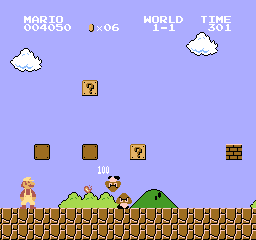
\includegraphics[width=0.45\textwidth]{FIG/SuperMarioBros.png} \\
\end{tabular}
\caption{
	슈퍼 마리오 브라더스의 게임 화면.
}
\label{fig:mario_title}
\end{center}
\end{figure}

슈퍼 마리오 브라더스는 닌텐도 초기의 액션 게임으로 1985년 9월 13일 NES (Nintendo Entertainment System) 전용 게임으로 출시 되었다.
Figure~\ref{fig:mario_title}은 이 게임의 플레이 화면이다.
당시 출시된 다른 게임들과 비교하여 우수한 조작감과 완성도 높은 미술로 크게 흥행하였으며 현재 2019년도 까지고 지속적으로 후속작이 출시되고 있다.
간단한 조작으로도 자유도 높은 플레이가 가능하여 강화학습의 목표로 삼기에 적합하여 이번 프로젝트의 대상으로 선택하였다.
슈퍼 마리오 브라더스는 총 8개의 world 와 각 world 당 4개의 stage로 구성되어 있다.
각 world 별로 특징있는 컨셉을 (물의 나라, 얼음의 나라, 등) 가지고 디자인 되어 배경 및 등장하는 적 케릭터가 차이가 있다.
또한 world 및 stage 수가 증가할 수록 난이도가 올라가는 경향을 가진다.

\begin{table}[]
	\caption {
		슈퍼 마리오 브라더스에서 가능한 키 입력. 서로 다른 키를 조합하여 입력하는 것이 가능하다.
	}
	\label{tab:mario:key}
\begin{tabular}{lr}
\toprule
키     & \multicolumn{1}{c}{동작 설명} \\
\midrule
up    & 특수한 상황(넝쿨, 파이프)에서 마리오를 위로 이동 \\
left  & 마리오를 왼쪽으로 이동 \\
down  & 특수한 상황(넝쿨, 파이프)에서 마리오를 아래로 이동 \\
right & 마리오를 오른쪽으로 이동 \\
A     & 가속 또는 불꽃 공격(슈퍼 마리오만 해당)\\
B     & 점프 \\
\bottomrule
\end{tabular}
\end{table}

Table~\ref{tab:mario:key} 에서 슈퍼 마리오 브라더스 게임에서 가능한 모든 키 입력을 소개한다.
모든 입력은 중복하여 입력하여 마리오가 다른 동작을 하게 할 수 있다.
예를 들면 right 키와 B 키를 동시에 입력하면 마리오가 오른쪽으로 나아가며 점프한다.
하지만 경우에 따라 right 키와 left 키를 동시에 누른 경우 처럼 상보적인 두 가지 키를 조합하는 경우 무의미한 동작을 나타낼 수도 있다.
슈퍼 마리오 브라더스 게임에서 유의미한 키조합을 고려할 경우 가능한 Action의 경우의 수는 16가지 이다.

슈퍼 마리오 브라더스에서 목적지인 깃발로 이동하면 한 stage가 종료된다.
그 외에는 적에게 부딧치거나, 함정에 빠진 경우, 그리고 제한 시간이 지난 경우 stage가 종료되며 처음부터 다시 시작하게 된다.
이 게임의 목적은 보다 많은 점수를 얻으면서 깃발에 도달하여 stage를 완료하는 것이다.
stage 내부에서 점수를 얻는 방법은 아래와 같다.
\begin{itemize}
	\item \textbf{깃발 도달시 남은 시간:}
		제한 시간 이내에 깃발에 도달한 경우 남은 시간 (초 단위)당 100점 획득.
	\item \textbf{동전을 획득:}
		stage내에서 벽돌, 물음표 블록, 그리고 동전 아이템을 통해 동전에 닿으면 100점 획득.
	\item \textbf{버섯, 꽃을 획득:}
		stage내의 물음표 블록에서 버섯 또는 꽃이 나왔을 때 닿으면 100점 획득.
	\item \textbf{적을 처치:}
		적을 처치시 기본적으로 100점 획득하며 연속된 처치를 할 경우 매번 2배의 추가 점수 획득.
\end{itemize}

이 게임에서 stage별로 목적지에 도달하지 못하고 종료된 경우 다시 도전할 기회를 부여하는 데 이 횟수는 마리오의 남은 생명으로 결정된다.
게임내에서 녹색 버섯을 획득하거나 동전을 100개 모은 경우 추가로 보너스 생명을 1개 얻게 된다.
강화학습을 위한 환경에서는 학습을 시키기 위해 stage를 수 많이 반복하여야 하여 이러한 재도전 횟수를 제한하는 것을 해제한 상태에서 학습시키게 된다.
하지만 실제 플레이어가 게임을 한다고 가정할 때 이러한 생명을 관리하는 것은 게임을 끝까지 완수하기 위한 중요한 요소이다.

\subsection{Basis for reinforcement learning}
강화학습에서 현재 state는 이 후 action을 결정하는 데 중요한 요소이다.
실제 게임 플레이어와 공평한 조건에서 경쟁하기 위해 본 프로젝트에서 state를 화면에 표시되는 이미지를 사용하여 결정하기로 하였다.
Convolutaionl neural network (CNN)~\cite{CNN}은 이미지로 부터 학습 모델에 필요한 feature를 추출하여 의사 결정에 활용하는 널리 알려진 방법이다.
본 프로젝트에서 우리는 화면 이미지를 CNN을 통해 해석하여 게임 점수를 최대한 얻을 수 있는 action을 추론하는 모델을 만들고자 한다.

우리는 키 조합을 통해 action을 생성할 수 있는데 유의미한 조합만을 고려하면 아래와 같은 16개의 키조합을 각각의 action으로 정의한다.
\begin{enumerate}
	\item 아무키도 누르지 않음
	\item left
	\item right
	\item up
	\item down
	\item A
	\item B
	\item A + B
	\item left + A
	\item left + B
	\item left + A + B
	\item right + B
	\item right + A
	\item right + A + B
	\item up + B
	\item down + B
\end{enumerate}
우리의 모델은 최종적으로 Figure~\ref{fig:overview}와 같이 현재 state에서 각 차원이 각 action에 대응되는 16차원의 vector를 산출하여 각 action의 적합성을 확률적으로 추론한다.
\begin{figure}[]
\begin{center}
\begin{tabular}{c}
     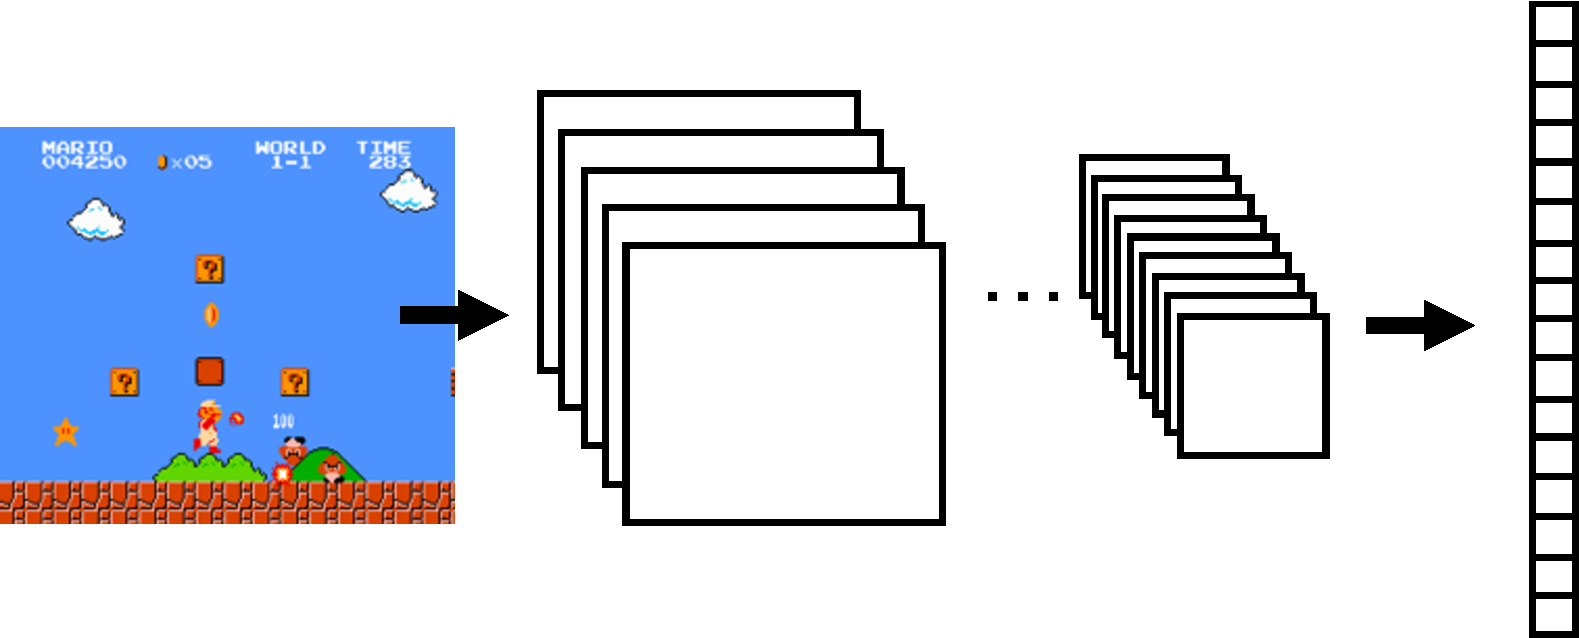
\includegraphics[width=0.45\textwidth]{FIG/overview.pdf} \\
\end{tabular}
\caption{
	게임 화면으로부터 action을 추론하기 위한 모델. CNN을 통해 게임화면을 해석하여 16차원의 action의 적합성을 추론한다.
}
\label{fig:overview}
\end{center}
\end{figure}

강화학습에서 모델은 현재 state에서 최종적으로 얻을 수 있는 reward를 극대화하는 action을 선택하도록 학습된다.
따라서 reward를 잘 설정해야 올바른 선택을 하도록 유도할 수 있다.
슈퍼 마리오 브라더스 게임에서 stage가 끝날 때 남은 시간당 100점을 획득하게 된다.
이는 다른 방법으로 얻는 점수보다 상당히 많은 양이다.
따라서 획득 점수 위주로 reward를 설정하였을 때, 마리오가 빠른 시간안에 깃발로 도달하도록 유도할 수 있다.
또한, stage 중간에 코인, 아이템, 그리고 적을 처치해서 얻는 점수를 고려하면 중간중간의 imediate reward로 활용되어 마리오가 해당 동작을 하도록 하는 학습을 할 수 있다.
이와 같이, stage 내부의 획득 점수를 통해 reward를 주는 것은 올바른 게임 플레이를 학습하는 데 도움을 준다.

게임의 특성상 마리오를 큰 마리오, 나아가 슈퍼 마리오로 변신시키면 남은 stage를 진행함에 있어 크게 유리한 요소로 작용한다.
우리 모델이 슈퍼 마리오로 변신하는 것을 지향하고 변신이 풀리는 것을 지양하기 위해 상위 단계로 변신할 때 획득 점수이외의 부가적인 reward를 할당하고, 변신이 풀릴 경우 reward를 크게 감소시키도록 한다.

\subsection{State from partial area}
사람들이 슈퍼 마리오 브라더스를 실제로 플레이할 때, 사람들은 상황에 따라 화면의 일부분을 좀 더 집중해서 바라보게 된다.
예를 들면, 마리오가 공중에서 하강하고 있을 때는 마리오의 아래 쪽에 집중하여 바닥의 함정을 피하거나 적을 밟아 처치하도록 조작한다.
전반적으로, 전체 화면의 내용보다 마리오 주변에서 일어나고 있는 일에 집중하는 경향이 있다.

\begin{figure}[]
\begin{center}
\begin{tabular}{c}
     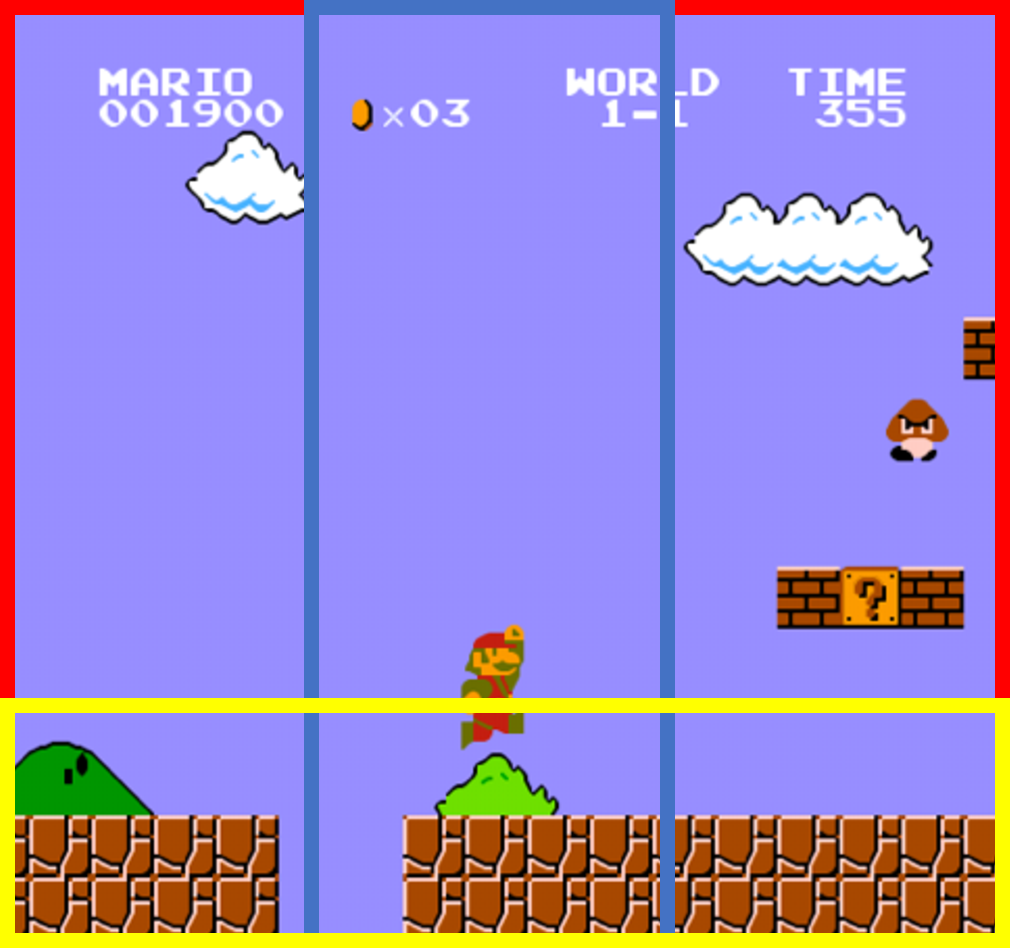
\includegraphics[width=0.4\textwidth]{FIG/split_screen.pdf} \\
\end{tabular}
\caption{
	화면 분할을 통해 여러 CNN 입력을 생성하는 예시. 전체 화면을 나타내는 빨간색, 마리오 주변을 나타내는 파란색, 그리고 바닥의 함정을 조심하기 위한 노란색 영역이 있다.
}
\label{fig:split_screen}
\end{center}
\end{figure}

이러한 게임의 특성을 고려하여 우리 모델도 여러 개의 CNN을 만들어 화면의 각 구역별로 따로 feature를 추출하기로 한다.
이렇게 추출한 feature의 중요도는 마리오의 상황에 따라 변화한다. 앞서 예와 같이 마리오가 공중에 있다면 마리오 주변에 좀 더 집중해야 한다.
만약 마리오의 달리기 속도가 빠른 상황이라면 좀 더 전체 화면부위를 고려하여 다음 action을 정해야한다.
또한 바닥의 함정에 빠지면 마리오가 즉사할 수 있으므로 아래 쪽 영역에 대한 주의도 늦출 수 없다.
우리 모델에서는 figure~\ref{fig:split_screen}과 같이 여러 구역으로 나눠 입력을 만든 후 각각의 CNN으로 생성된 feature를 마리오의 현재 상황에 따라 중요도를 계산하도록 attention layer를 통해 현재 feature를 결정하도록 한다.


